\documentclass[class=book, crop=false, oneside]{standalone}
\usepackage[subpreambles=true]{standalone}

\usepackage{../../style}

\graphicspath{{./assets/images/}}

% arara: pdflatex: { synctex: yes, shell: yes }
% arara: latexmk: { clean: partial }
\begin{document}
\chapter{Central Processing Unit}

\section{Introduzione}
In questo capitolo andremo ad analizzare come il nostro processore elabora ed esegue le istruzioni che gli arrivano dai programmi Assembly; in particolare ci baseremo ancora su MIPS, in quanto super regolare e particolarmente utile a scopo didattico.\\
Per come è stato progettato MIPS, le istruzioni presentano dei tratti comuni; in particolare le prime due fasi del ciclo della CPU (vedi~\ref{subsec:cpu}): il prelievo dell'istruzione e la lettura dei valori dei registri operandi sono comuni a ogni istruzione.\\
Noi in particolare, dopo aver spiegato i vari elementi che concorrono a far funzionare tutta la baracca, andremo ad analizzare le istruzioni aritmetico-logiche, quelle di accesso alla memoria e quelle di salto, dal momento che tutte le altre si implementano con tecniche simili.

\section{Arithmetic-Logic Unit}
A eccezione di \opcode{j}, tutte le istruzioni MIPS fanno uso di \emph{arithmetic-logic unit} (ALU per gli amici), una rete logica combinatoria abbastanza complessa preposta all'esecuzione di tutti calcoli di cui abbiamo bisogno; sostanzialmente, è un’unione di blocchi fondamentali che fanno operazioni su singoli bit.\\
Al di là delle operazioni puramente aritmetiche (per le quali lo scopo di ALU è ovvio), viene usata nelle operazioni di accesso alla memoria (\opcode{sw} e \opcode{lw}) per il calcolo degli indirizzi e dalle operazioni di salto condizionato per effettuare i confronti; successivamente, ognuna di queste tre categorie differisce.

\section{Il datapath}
Il \emph{datapath} è quella parte del processore attraverso cui passano le istruzioni; è letteralmente un percorso da seguire ogniqualvolta si voglia esegire una qualsiasi istruzione.

\subsection{Struttura del datapath}
\begin{figure}[H]
	\centering
	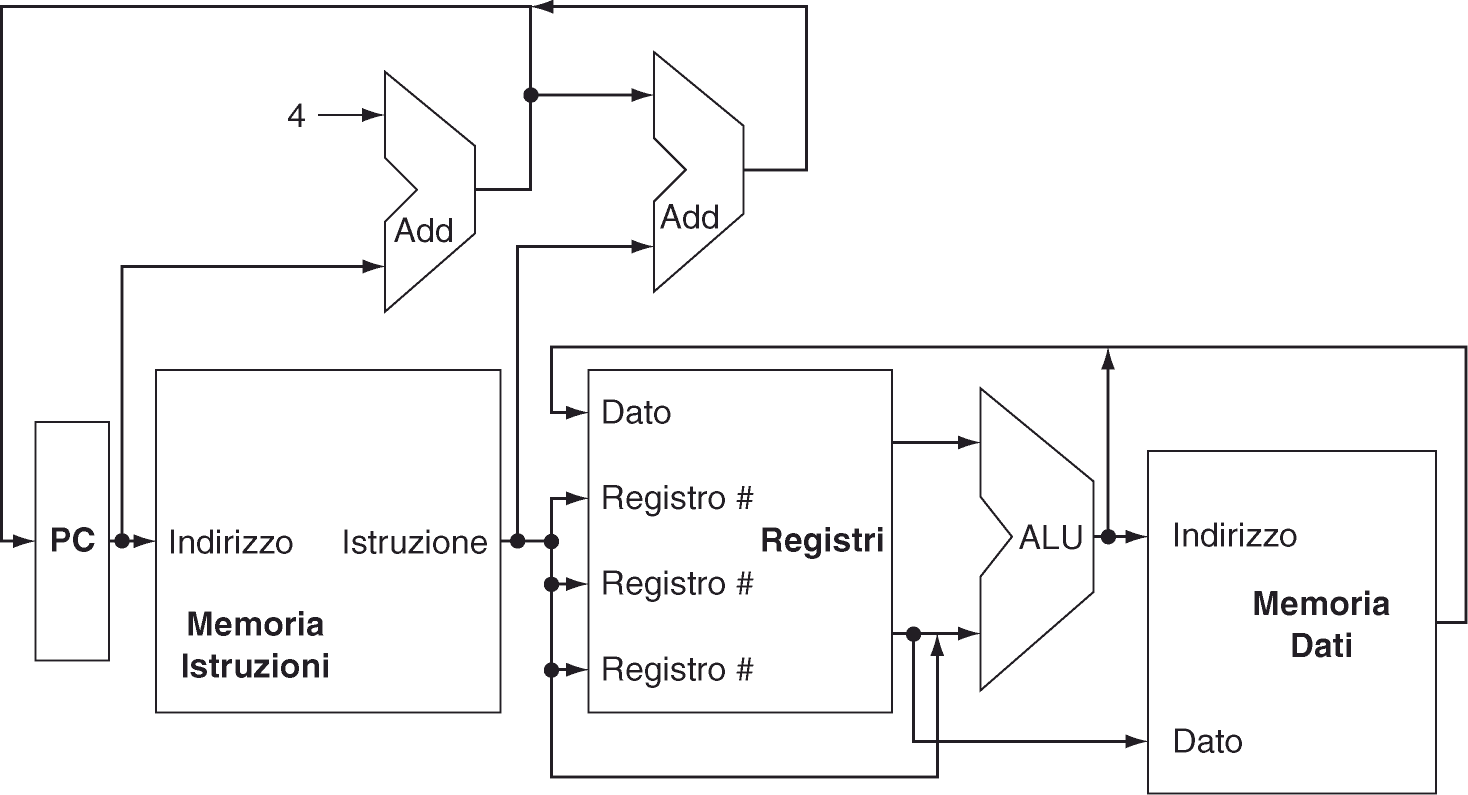
\includegraphics[width=0.9\textwidth,keepaspectratio]{datap_1}
	\caption{Schema base del datapath}
\end{figure}
Il datapath si compone essenzialmente di 5 fasi:
\begin{enumerate}
  \item Assumendo che il programma sia già stato caricato in memoria (secondo le modalità viste nel capitolo~\ref{ch:tool}), in questa fase viene prelevata l'istruzione da eseguire e viene spacchettata nei vari campi;
  \item I registri interessati all'esecuzione vengono caricati nel \emph{banco dei registri}; se l'istruzione è di tipo R, gli indirizzi dei registri sono contenuti nel corpo dell'istruzione;
  \item A questo punto la ALU esegue i calcoli opportuni, ottenendo il valore (o l'indirizzo) desiderato;
  \item I risultati ALU vengono utilizzati per salvare (o prelevare) in memoria dati un dato, o per memorizzare un registro;
  \item Si incrementa il \emph{PC} per mezzo di una ALU dedicata (di fatto, un addizionatore), e una successiva ALU calcola l’indirizzo verso cui ci si deve spostare in caso di salti incondizionati.
\end{enumerate}

\subsection{Il ruolo del multiplexer}
La  figura però è incompleta; manca qualcosa che dica ai blocchi cosa fare in caso di punti di decisione (momenti in cui i segnali arrivano da due diverse sorgenti e bisogna sceglierne una), come ad esempio l'incremento del program counter: normalmente, il suo valore proviene dall'addizionatore (e punta quindi alla word successiva a quella appena letta), ma in caso di salto l'indirizzo viene calcolato dallo spiazzamento contenuto nell'istruzione.\footnote{Si ricorda che MIPS offre  solo 16 bit per immagazzinare costanti all'interno di istruzioni immediate. Dunque, attraverso \opcode{beq} risulta necessario utilizzare riferimenti relativi (al \(\textrm{\emph{PC}}+4\)) e non assoluti per poter accedere ad una vasta gamma di indirizzi.} Altro esempio: a seconda della tipologia di istruzione il secondo operando della ALU potrà provenire o dal banco dei registri (per le istruzioni R) o dal codice dell'istruzione stessa (per le istruzioni I).

Ed è qui che ci viene in soccorso il \emph{multiplexer} che, come già detto in~\ref{subsec:multi}, è un circuito combinatorio che prende in input due segnali e decide quale di essi debba andare in output sulla base di un terzo segnale di controllo (un po' come un vigile che decide quale macchina far passare).
\begin{figure}[H]
	\centering
	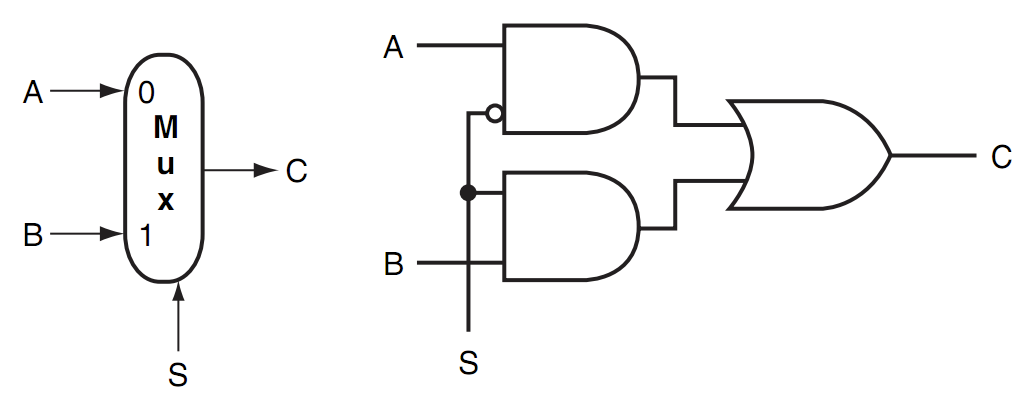
\includegraphics[width=0.8\textwidth,keepaspectratio]{multi}
	\caption{Schema di un multiplexer}
\end{figure}
\paragraph{Altri elementi}
Oltre ai multiplexer, ci sono altri elementi che concorrono alla soluzione dei punti di decisione. Ad esempio, la ALU viene notificata con un segnale di controllo (nel nostro caso di \(4\) bit) per decidere quale operazione effettuare, il banco dei registri riceve dei flag per decidere se scrivere o meno un registro, la memoria dati ha degli espedienti per decidere se effettuare lettura o scrittura, e simili.\\
Chi stabilisce queste cose, oltre a settare il segnale del selettore dei vari multiplexer? È presto detto, l’unità di controllo!\\

\section{La Control Unit}
La \emph{Control Unit} funge da vero e proprio "direttore d'orchestra" per il processore, stabilendo il valore \(S\) dei vari multiplexer e andando a sciogliere le questioni dei punti di decisione.
\begin{figure}[H]
	\centering
	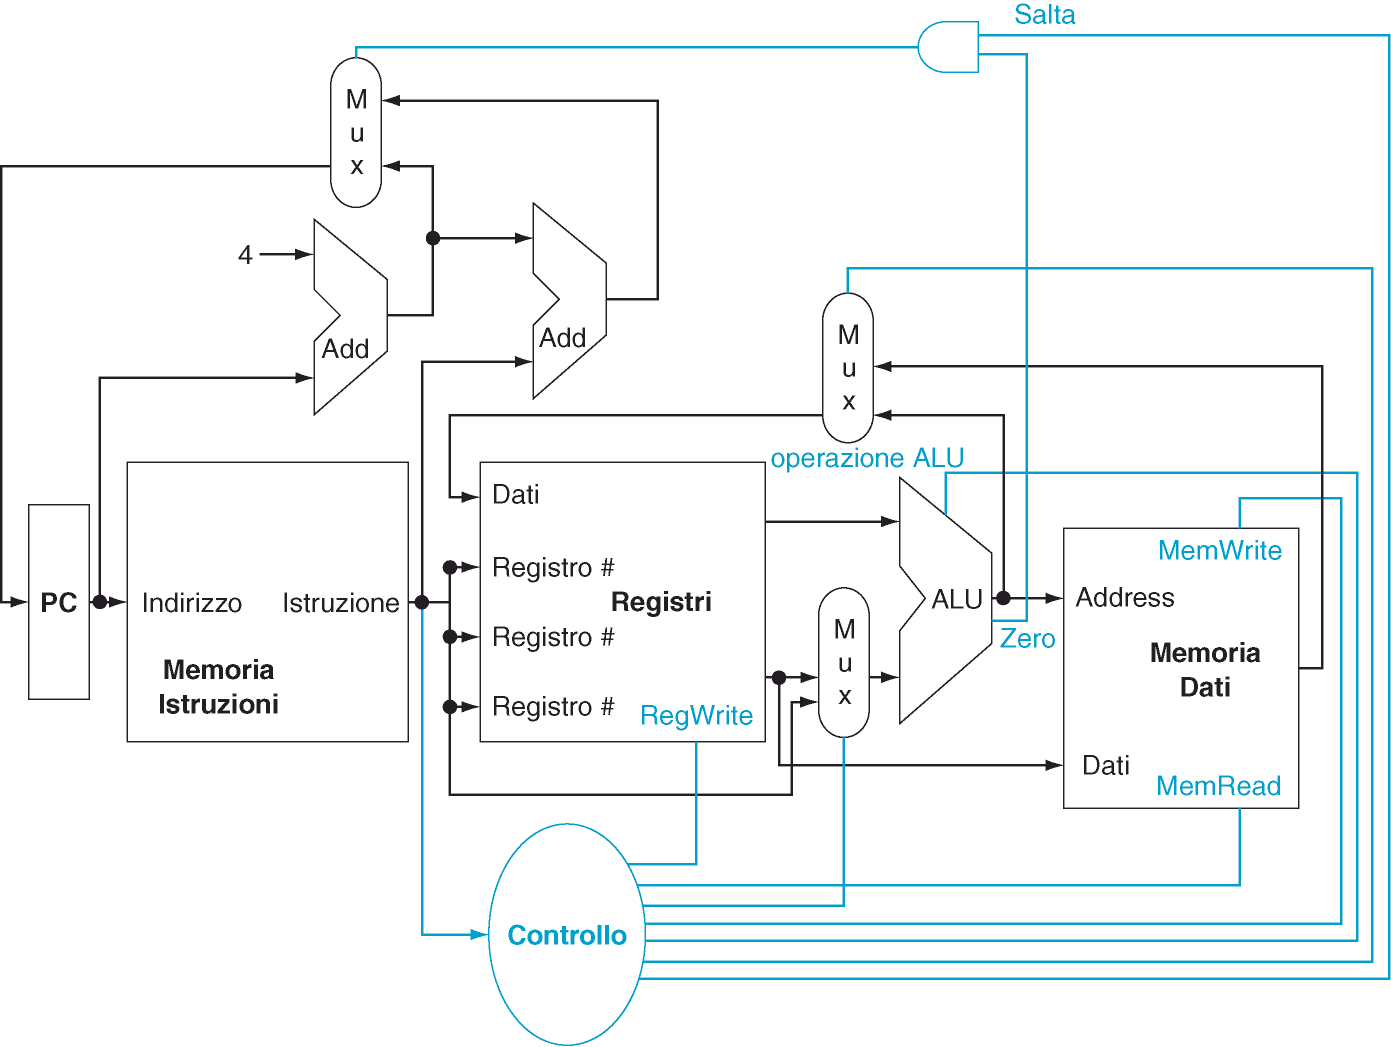
\includegraphics[width=0.9\textwidth,keepaspectratio]{datap_2}
	\caption{Schema di datapath e control unit}
\end{figure}
La figura è molto complessa, andiamo ad analizzarla con ordine.
\begin{itemize}
	\item Innanzitutto notiamo il multiplexer prima del \emph{PC}: questo gestisce la scelta su come viene aggiornato il \emph{PC}, se secondo il valore del primo o del secondo addizionatore. Per settare il valore \(S\) viene utilizzata una porta AND, il cui primo input arriva direttamente dalla control unit, mentre il secondo viene fornito dalla ALU (\emph{zero}).
	\item Vediamo un secondo multiplexer che indica se memorizzare nel registro di destinazione un dato da ALU o dalla memoria.
	\item Abbiamo un  ultimo multiplexer che precede il caricamento del secondo operando nell'ALU: dalla control unit arriverà l'indicazione per scegliere di caricare un registro (nelle istruzioni R) o una costante (per quelle I).
	\item Poi vediamo un segnale per la ALU: esso consiste di un bus di più bit per comunicare all'unità quale operazione eseguire.
	\item Alla memoria dati invece arrivano i segnali \emph{MemWrite} e \emph{MemRead}, che indicano alla memoria dati  la rispettiva operazione.
	\item In base al valore di \emph{RegWrite}, il risultato dell'operazione viene memorizzato nel registro di destinazione.
\end{itemize}

Questa è la rappresentazione di MIPS, che è una ISA RISC; inutile dire che gli schemi di funzionamento che stanno alla base di architetture CISC sono incredibilmente più complessi di così.

\section{La temporizzazione}
A questo punto abbiamo moltissimi segnali che viaggiano nel processore, sincronizzati dal clock. Per semplicità assumiamo che tutte le istruzioni vengano eseguite con un ipotetico singolo colpo di clock lungo abbastanza.

\subsection{Breve riepilogo sulle reti logiche}
Circuiti come i multiplexer sono detti \emph{reti combinatorie} e producono un output secondo una funzione statica dell'input, senza memoria dei cambiamenti.\\
Risulta però chiaro che elementi come i registri e le memorie (detti elementi "di stato") necessitano di tenere traccia dei cambiamenti subiti. In questo caso giungono in nostro soccorso le \emph{reti sequenziali}, dove l'output dipende dalla storia (sequenza) degli input precedenti. Si ha inoltre che gli elementi di stato hanno almeno due ingressi:
\begin{itemize}
	\item il valore da immettere nello stato;
	\item il clock atto a sincronizzare le transizioni.
\end{itemize}

\paragraph{Flip-flop}
Il \emph{flip-flop D-latch} è l’elemento base per memorizzare un bit, e registri sono di fatto vettori di vettori di 32 di questi circuiti (rivedi~\ref{subsec:latch} per maggiori dettagli).

\subsection{Gestione della temporizzazione}
Avere un clock regolare ci permette di ottenere indicazioni precise sulla sequenza di operazioni svolte e avere sempre ragione di quale istruzione è avvenuta prima o dopo di un determinato colpo di clock. La metodologia di temporizzazione ci dà quindi indicazioni precise rispetto alla possibilità di lettura/scrittura dei segnali rispetto al clock, e i dati presi dagli elementi di stato sono sempre relativi ai cicli precedenti. Vediamo uno schema di come viene gestita la cosa:
\begin{figure}[H]
	\centering
	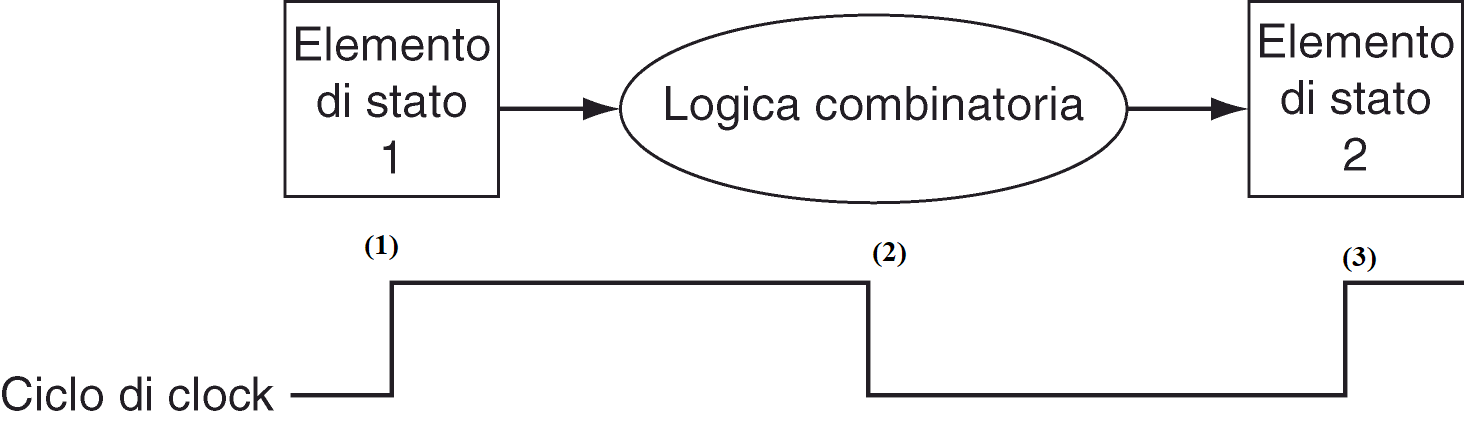
\includegraphics[width=0.6\textwidth,keepaspectratio]{clock}
\end{figure}
\begin{enumerate}
	\item l'elemento di stato 1 viene aggiornato a un determinato tempo \(t\);
	\item il valore passa attraverso a una qualsiasi rete combinatoria;
	\item il valore arriva all'elemento di stato 2 al tempo \(t + T\).
\end{enumerate}
Il tempo \(T\) di clock deve naturalmente essere tale da dare tempo ai valori di attraversare i vari circuiti combinatori; inoltre il periodo del clock ci permette di regolarizzare quelli che altrimenti diventerebbero dei cicli di retroazione assolutamente non predicibili.
\begin{figure}[H]
	\centering
	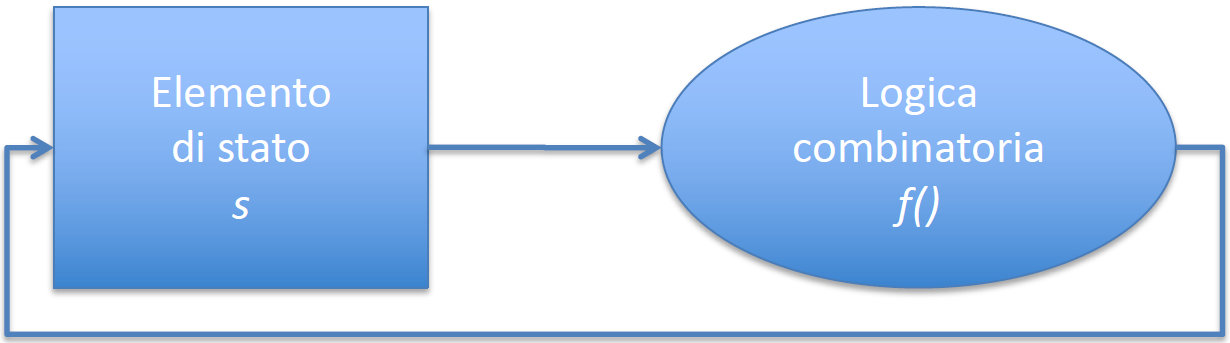
\includegraphics[width=0.5\textwidth,keepaspectratio]{retroaz}
\end{figure}
Se non avessimo una metodologia di temporizzazione precisa avremmo che \(s = f(s)\), che è un risultato assolutamente non prevedibile. Grazie alla temporizzazione sensibile al clock possiamo ottenere un andamento del tipo: \(s(t + T) = f(s(t))\), decisamente più regolare ed efficiente per noi poichè deterministico e non più afflitto da incertezza.

\section{Elaborazione delle istruzioni}
Prima di addentrarci nel dettaglio dell'esecuzione di alcuni tipi di istruzioni, passiamo in rassegna le varie componenti che servono alla realizzazione di un datapath:
\begin{figure}[H]
	\centering
	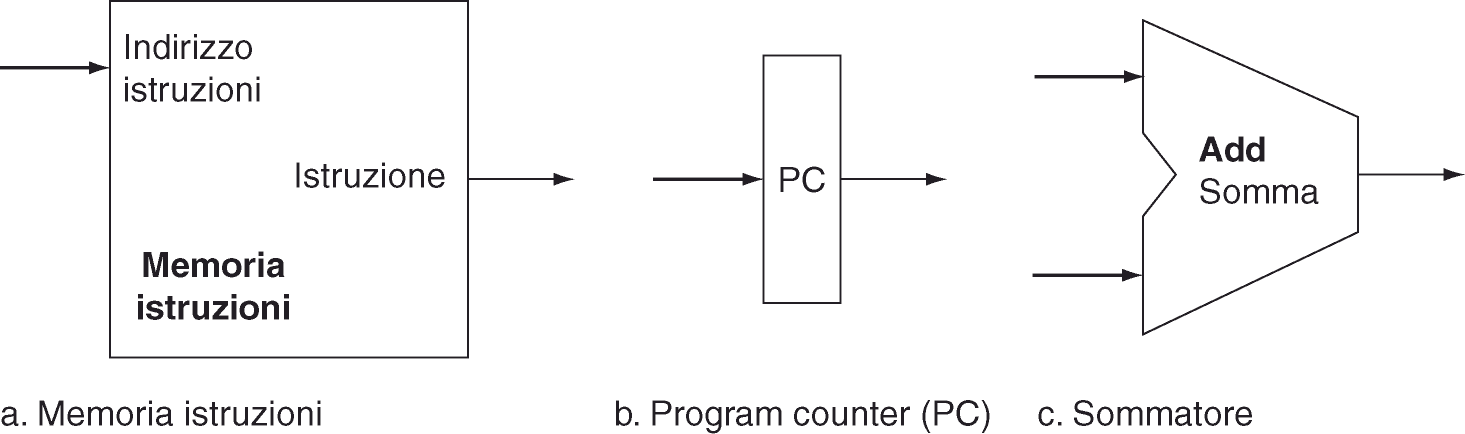
\includegraphics[width=0.9\textwidth,keepaspectratio]{datap_3}
\end{figure}
Ricordiamo che il sommatore (o addizionatore) è una ALU specializzata alla sola operazione di incremento del \emph{PC}.\\
A questo punto la fase di fetch, ricordiamolo, prevede il prelievo dell'istruzione dal \emph{PC}, il trasferimento della stessa agli elementi proposti all'esecuzione e l'incremento del \emph{PC}.

\subsection{Istruzioni R}
Iniziamo con un’istruzione di tipo R, come potrebbe essere:
\begin{minted}[linenos]{asm}
add $t0, $s1, $s2
\end{minted}
la quale, come sappiamo, ha questo tipo di mapping:
\begin{figure}[H]
	\centering
	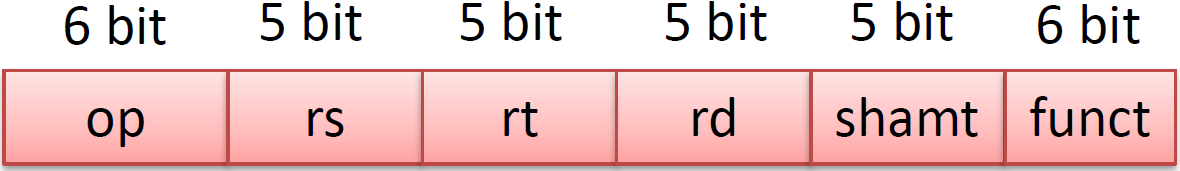
\includegraphics[width=0.5\textwidth,keepaspectratio]{mappatura.png}
\end{figure}
Per effettuare questa operazione abbiamo bisogno di due blocchi funzionali che vanno ad aggiungersi ai tre di base che abbiamo visto prima.
\begin{figure}[H]
	\centering
	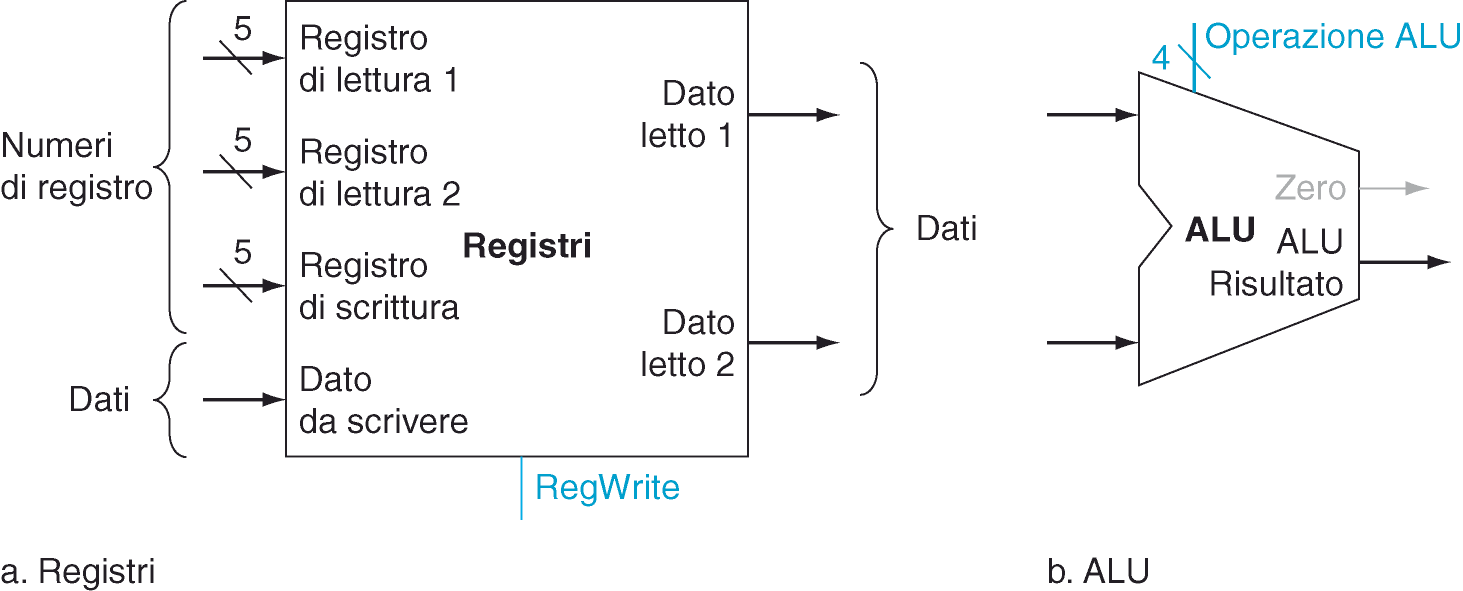
\includegraphics[width=0.8\textwidth,keepaspectratio]{R_ex.png}
\end{figure}
\begin{itemize}
	\item Il primo blocco è il \emph{banco dei registri}, una struttura con 3 bus da 5 bit ciascuno in cui vengono caricati i registri da operare; per decidere se dovrò leggere o scrivere un determinato registro viene impiegato il controllo \emph{RegWrite}, gestito direttamente dalla Control Unit.
	\item Il secondo blocco di cui abbiamo bisogno è la ALU di cui prima abbiamo tanto parlato. Questa presenta due controlli: uno di questi è il bus che arriva dal corpo dell'istruzione e indica qual è l'operazione da svolgere, mentre il secondo è il settaggio \emph{zero} qualora il risultato dell'operazione fosse effettivamente 0; quest'ultimo valore viene poi mandato alla porta AND che decide il segnale di controllo per il multiplexer preposto alla scelta del blocco d'incremento del \emph{PC}.
\end{itemize}

\subsection{Istruzioni di accesso alla memoria}
Adesso andiamo ad analizzare le seguenti istruzioni sulla memoria:
\begin{minted}[linenos]{asm}
lw $t0, offest($t2)
sw $t0, offest($t2)
\end{minted}
Ricordiamo che presentano la seguente mappatura:
\begin{figure}[H]
	\centering
	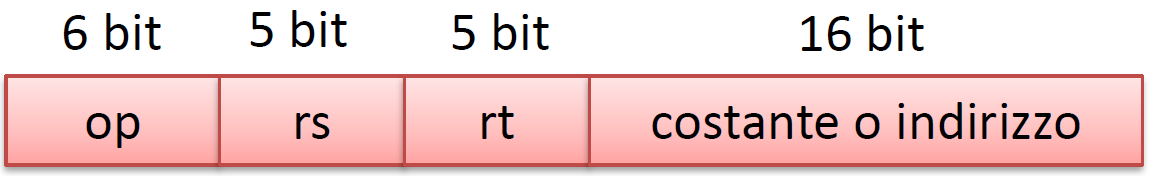
\includegraphics[width=0.5\textwidth,keepaspectratio]{I.png}
\end{figure}
In entrambi i casi avremo bisogno di calcolare l'indirizzo in memoria dato da \register{\$t2} e dallo spiazzamento, per cui ci servirà nuovamente una ALU.
\begin{figure}[H]
	\centering
	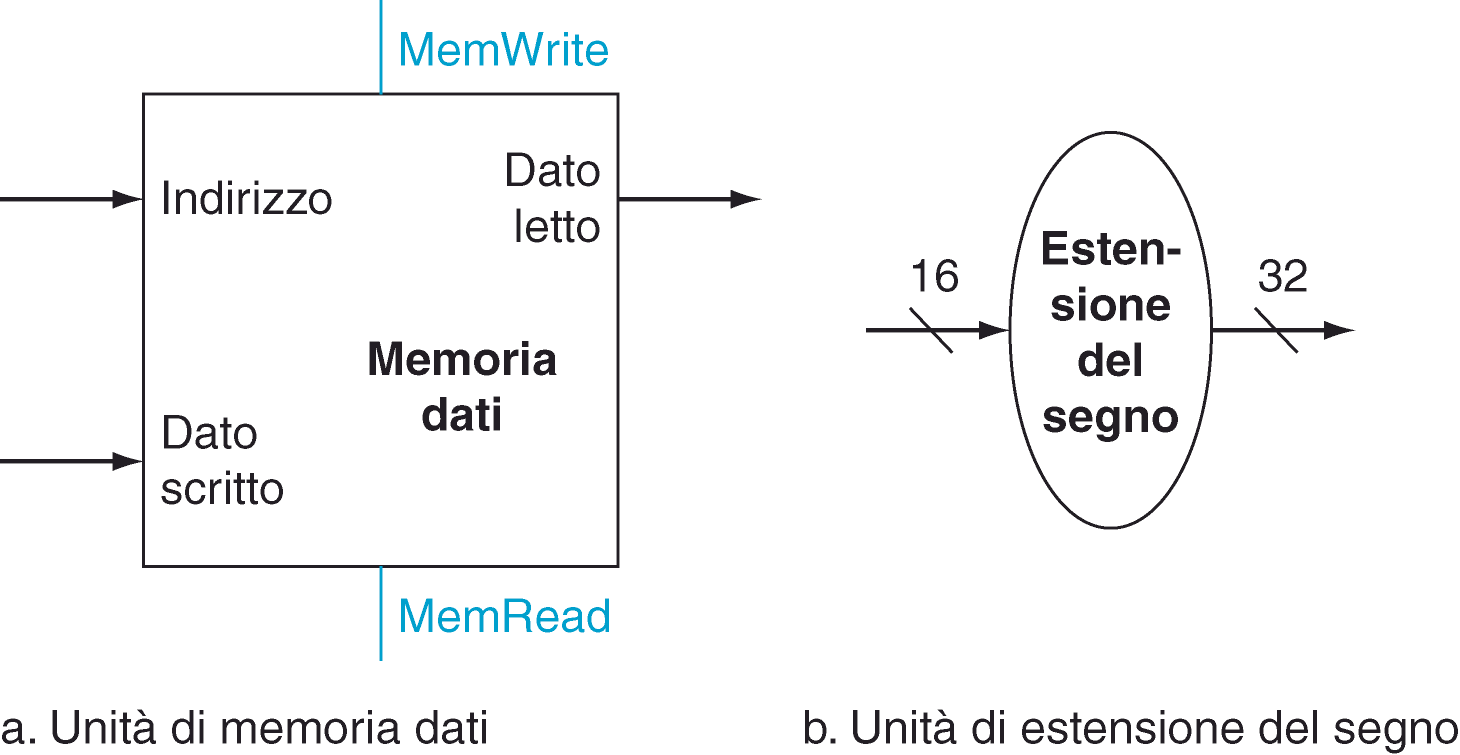
\includegraphics[width=0.65\textwidth,keepaspectratio]{MemAccess.png}
\end{figure}
In aggiunta:
\begin{itemize}
	\item avremo bisogno di una \emph{memoria dati}, dove eventualmente potremo memorizzare i dati di \mintinline{asm}{sw};
	\item abbiamo bisogno di due segnali di controllo appositi per indicare se l'operazione da eseguire è di lettura o scrittura;
	\item osserviamo che l'offset viene memorizzato in un campo a 16 bit che potrebbe essere necessario estendere a 32 bit replicando per 16 volte il bit di segno: per questo abbiamo bisogno di un blocco funzionale apposito.
\end{itemize}

\subsection{Istruzioni di salto condizionato}
Andiamo ora a vedere la seguente istruzione:
\begin{minted}[linenos]{asm}
beq $t1, $t2, offset
\end{minted}
Ovviamente anche qui bisogna sommare l'offset, per cui di nuovo necessitiamo di una ALU. Osserviamo inoltre che il \emph{PC} viene incrementato di 4 byte ogni ciclo, per cui quando effettuiamo un salto andiamo a riferire l'offset al \emph{PC} già incrementato; inoltre MIPS shifta automaticamente gli indirizzi di istruzioni a sinistra di 2 bit, in modo da ragionare sempre in words ed espandere in numero di indirizzi raggiungibili.
\begin{figure}[H]
	\centering
	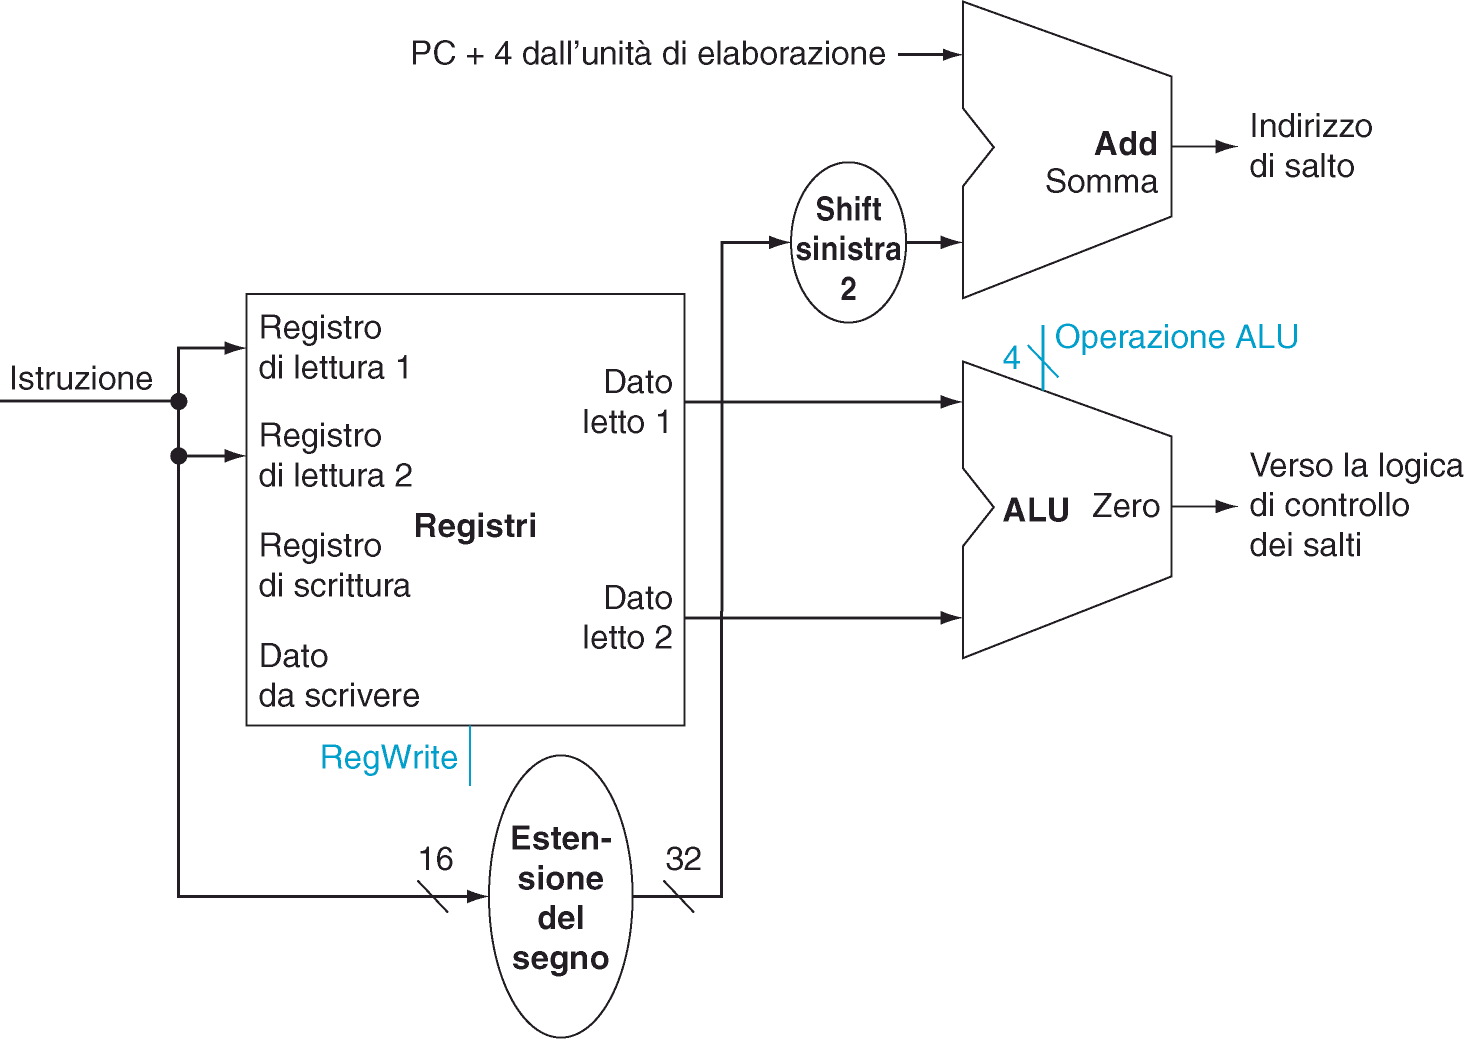
\includegraphics[width=0.7\textwidth,keepaspectratio]{jump.png}
\end{figure}
Dallo schema emergono:
\begin{itemize}
	\item una prima ALU, preposta al calcolo dell'indirizzo di salto da comunicare al \emph{PC};
	\item una seconda ALU, che effettua una sottrazione fra i due valori in ingresso. Se il risultato è 0 (e quindi i due sono uguali) lo comunica, insieme ad un segnale che indica l'avvenimento di una istruzione di branch, alla porta AND. Il risultato di quest'operazione logica verrà infine inviata al multiplexer che si occupa di selezionare correttamente il valore del nuovo \emph{PC}. In particolare:
	\begin{itemize}
		\item se l'AND risulta 0, \(\textrm{\emph{PC}}=\textrm{\emph{PC}}+4\);
		\item se l'AND risulta 1, \(\textrm{\emph{PC}}=\textrm{\emph{PC}}+4+\textrm{ind\_relativo}\), dove \emph{ind\_relativo} è l'indirizzo relativo all'istruzione a cui effettuare il \opcode{beq}.
	\end{itemize}
\end{itemize}

\section{Prima progettazione completa di una CPU}
Dopo aver visto in generale quali sono le principali componenti di una CPU e il loro funzionamento di base, possiamo cimentarci nella progettazione di una CPU completa.\\
Uno dei prerequisiti fondamentali per la nostra CPU è quello di essere in grado di eseguire ciascuna operazione in un singolo ciclo di clock: risulta perciò impossibile utilizzare una singola unità funzionale più di una volta all'interno di uno stesso ciclo. Proprio per questo motivo, come abbiamo visto, la memoria viene divisa in due: una zona viene dedicata alle istruzioni, l'altra ai dati.\\
In aggiunta, la nostra CPU dovrà implementare alcune semplici istruzioni aritmetico/logiche (\opcode{add}, \opcode{sub}, \opcode{and}, \opcode{or} e \opcode{slt}), istruzioni di lettura e scrittura in memoria (\opcode{lw} e \opcode{sw}) e istruzioni di salto (condizionato nel caso di \opcode{beq} e non condizionato nel caso di \opcode{j}).

\begin{figure}[H]
	\centering
	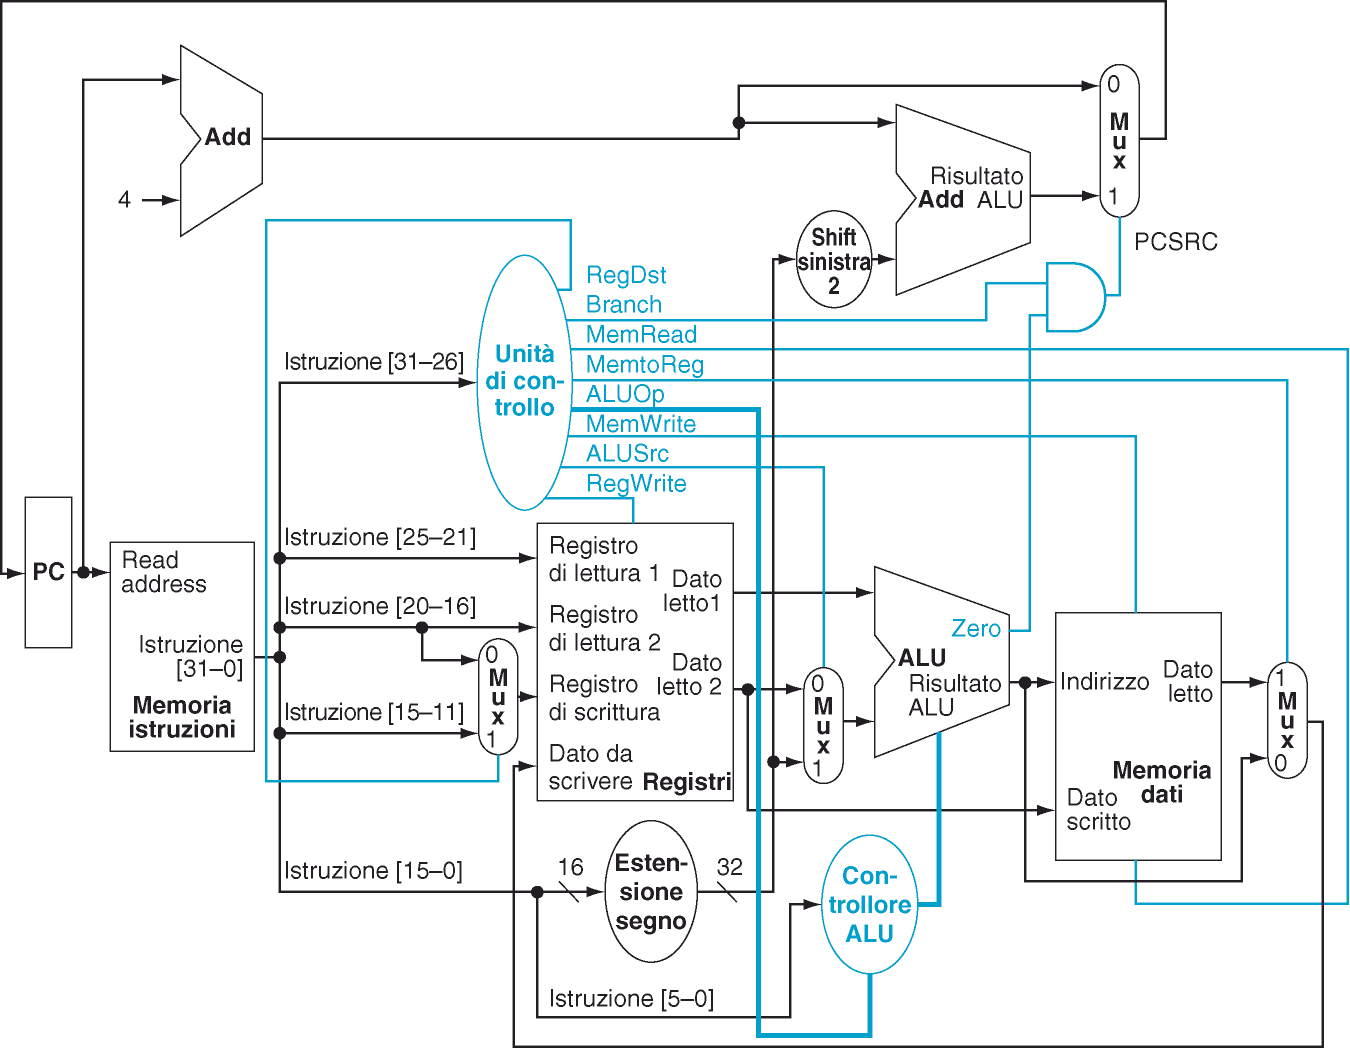
\includegraphics[width=0.95\textwidth,keepaspectratio]{schema_complessivo.png}
	\caption{Schema complessivo di un'unità di elaborazione}
\end{figure}
Anche se ne parleremo più approfonditamente in futuro, da questa rappresentazione è già possibile notare come varino i segnali di controllo in base al tipo di istruzione che viene eseguita. Ad esempio:
\begin{itemize}
	\item con istruzioni di tipo R: \(\textrm{\CUflag{ALUSrc}}=1\), \(\textrm{\CUflag{REGwrite}}= 1\), \(\textrm{\CUflag{MemtoReg}}=0\);
	\item con istruzioni \opcode{lw}: \(\textrm{\CUflag{ALUSrc}}=1\), \(\textrm{\CUflag{REGwrite}}= 1\), \(\textrm{\CUflag{MemtoReg}}=1\).
\end{itemize}

\subsection{Progettazione dell'unità di controllo della ALU}
L'\emph{unità di controllo della ALU} è una rete logica combinatoria che ha lo scopo di informare la ALU riguardo al tipo di operazione da eseguire sui dati ricevuti come input. Questo è possibile solamente se viene assegnato ad ogni istruzione un codice univoco (che nella nostra CPU sarà a 4 bit), chiamato \emph{codice di controllo ALU}.

\begin{table}[!h]
	\centering
	\subimport{assets/tables/}{codice_controllo_ALU}
	\caption{Istruzioni con il rispettivo codice di controllo ALU}
\end{table}
Definiamo più chiaramente il codice di controllo ALU: esso viene calcolato dall'unità di controllo della ALU attraverso il campo \emph{funct} (vedi~\ref{subsec:campiIstruzione}) e il codice \CUflag{ALUOp} dell'istruzione considerata. Brevemente:
\begin{itemize}
	\item \emph{funct}: corrisponde ai 6 bit meno significativi della rappresentazione in binario di un'istruzione MIPS;
	\item \emph{ALUOp}: consiste in 2 bit che permettono di categorizzare l'istruzione in base al suo tipo. Essa viene generata dall'unità di controllo centrale e assume i seguenti valori:
	\begin{itemize}
		\item 00: somma per istruzioni \opcode{lw} e \opcode{sw};
		\item 01: sottrazione per \opcode{beq};
		\item 10: operazione di tipo R.
	\end{itemize}
\end{itemize}
Questo processo non è da considerarsi indifferente: in questo modo è possibile utilizzare solo 4 bit per indicare all'ALU quale operazione eseguire, piuttosto che degli 8 bit inzialmente necessari (rispettivamente 6 per il campo \emph{funct} e 2 per il codice di controllo \CUflag{ALUOp}).

A seguire vengono presentate delle tabelle che esplicitano la rappresentazione delle istruzioni considerate sia nella rappresentazioni a 4 bit che a 8\footnote{I valori dove sono presenti le 'X' non vengono considerati}.

\begin{figure}[H]
	\centering
	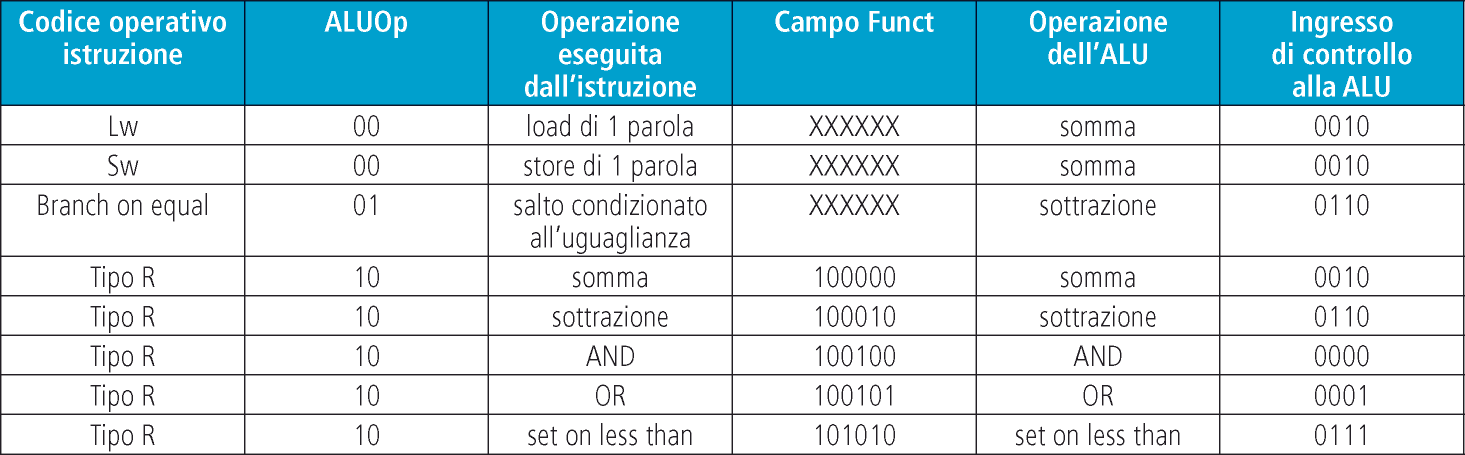
\includegraphics[width=0.95\textwidth,keepaspectratio]{riassunto_controllo_ALU.png}
	\caption{Generazione del codice di controllo ALU}
\end{figure}

\begin{figure}[H]
	\centering
	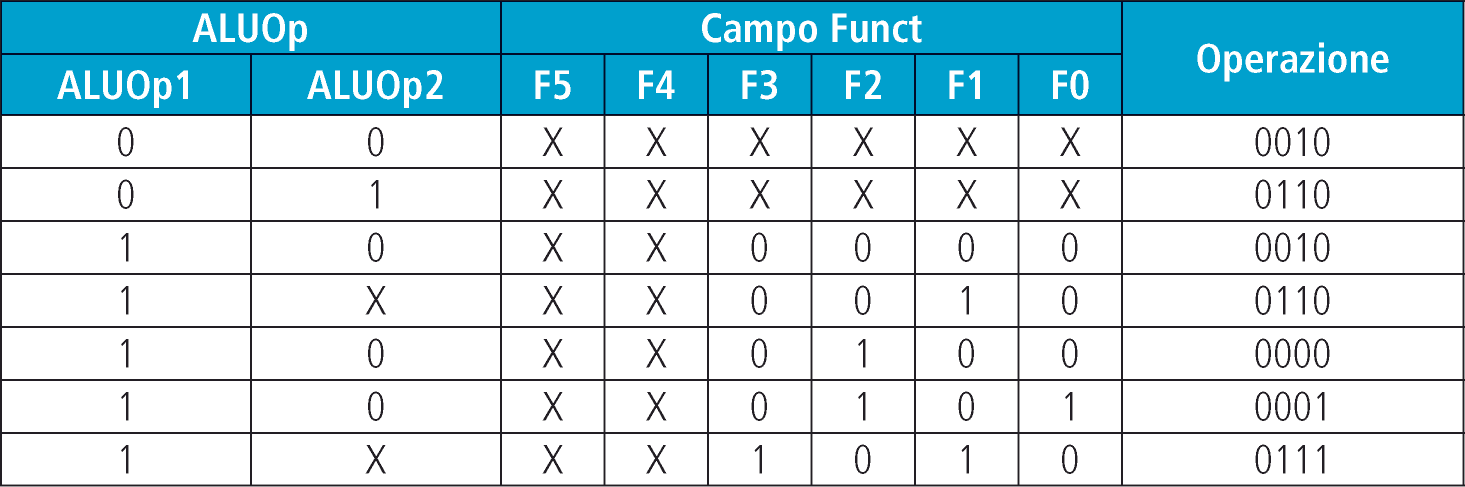
\includegraphics[width=0.80\textwidth,keepaspectratio]{tabella_verita_controllo_ALU.png}
	\caption{Tabella verità dell'unità di controllo ALU}
\end{figure}
Tirando le somme, quello che abbiamo appena visto è un sistema di decodifica e generazione dei comandi detto \emph{a due livelli}:
\begin{itemize}
	\item \emph{livello 1}: l'unità di controllo genera i segnali di controllo \CUflag{ALUOp} per l'unità di controllo della ALU;
	\item \emph{livello 2}: l'unità di controllo ALU genera i segnali di controllo per la ALU.
\end{itemize}

\subsection{Progettazione dell'unità di controllo principale}
L'\emph{unità di controllo principale} è una rete combinatoria che prende come input il codice operativo (in termini tecnici \emph{opcode}, vedi~\ref{subsec:campiIstruzione}) dell'istruzione caricata e genera i segnali di controllo appropriati. A seguire un elenco dei principali segnali di controllo e dei loro effetti collaterali:

\begin{figure}[H]
	\centering
	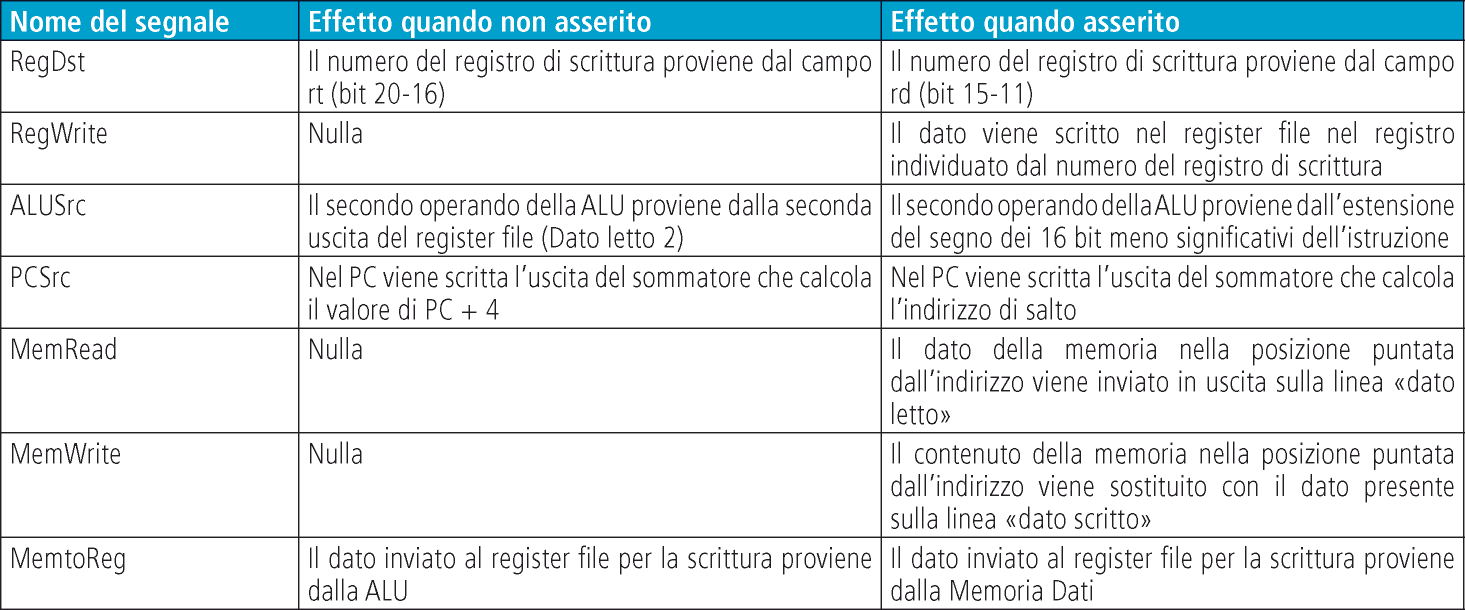
\includegraphics[width=0.95\textwidth,keepaspectratio]{segnali_controllo.png}
	\caption{Segnali unità di controllo principale}
\end{figure}
Elenchiamo ora, per le istruzioni che abbiamo intenzione di implementare, il valore che assumono i segnali di controllo prodotti dall'unità di controllo principale:

\begin{figure}[H]
	\centering
	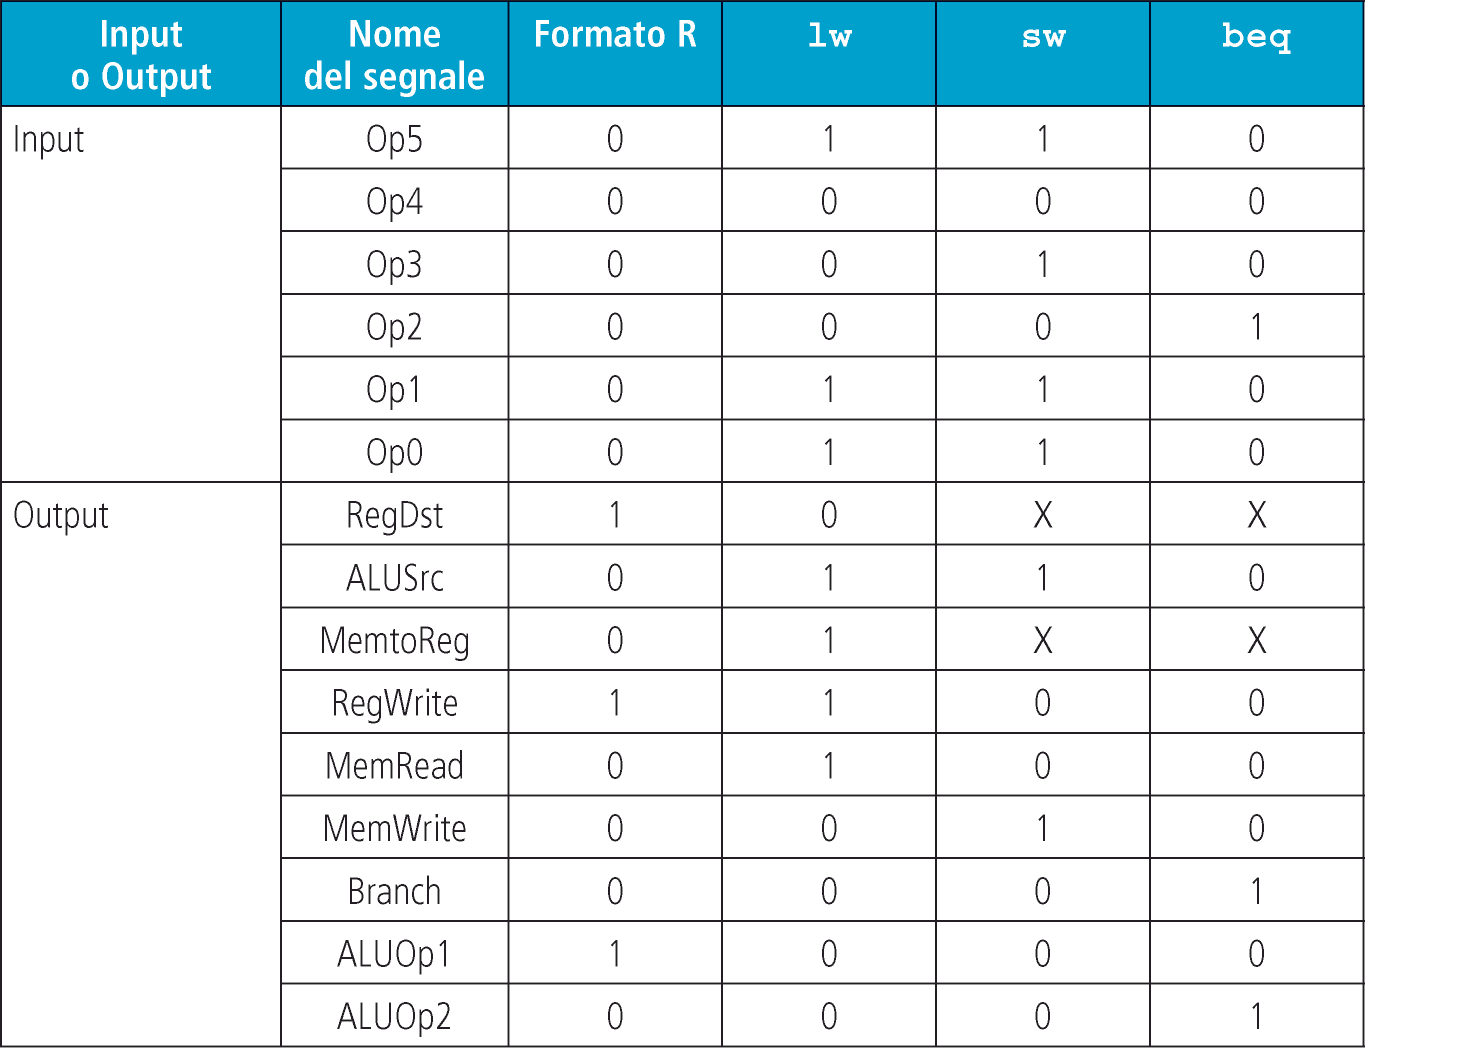
\includegraphics[width=0.80\textwidth,keepaspectratio]{io_CU.png}
	\caption{Schema complessivo di I/O di una CU principale}
\end{figure}
Lasciamo al lettore un ulteriore schema riassuntivo, in cui rimarchiamo ancora una volta la struttura delle istruzioni MIPS codificate in binario. Si noti che la prima colonna di questa tabella, ossia i 6 bit più significativi, corrispondono all'\emph{opcode}:
\begin{figure}[H]
	\centering
	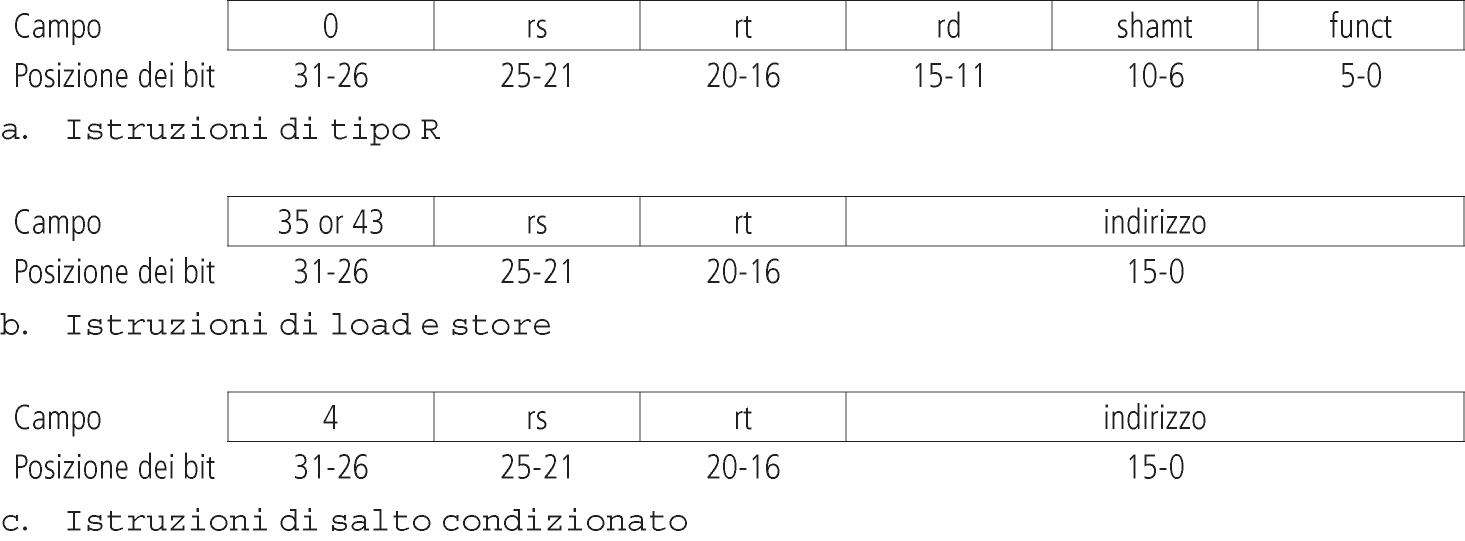
\includegraphics[width=0.80\textwidth,keepaspectratio]{campi_istruzione.png}
	\caption{Campi istruzione}
\end{figure}

\subsection{Esecuzione delle principali istruzioni}

\subsubsection{Istruzione di ADD}
Per eseguire un'istruzione di somma del tipo \mintinline{asm}{add $t1, $t2, $t3}, occorre:
\begin{enumerate}
	\item Prelevare l’istruzione dalla memoria e incrementare il \register{PC} di 4;
	\item Leggere \register{\$t2} e \register{\$t3} dal register file;
	\item Attivare la ALU con in input i dati dal register file;
	\item Memorizzare il risultato nel registro destinazione.
\end{enumerate}
Si ricordi che l'insieme di tutte queste operazioni va eseguito in un unico ciclo di clock.

\begin{figure}[H]
	\centering
	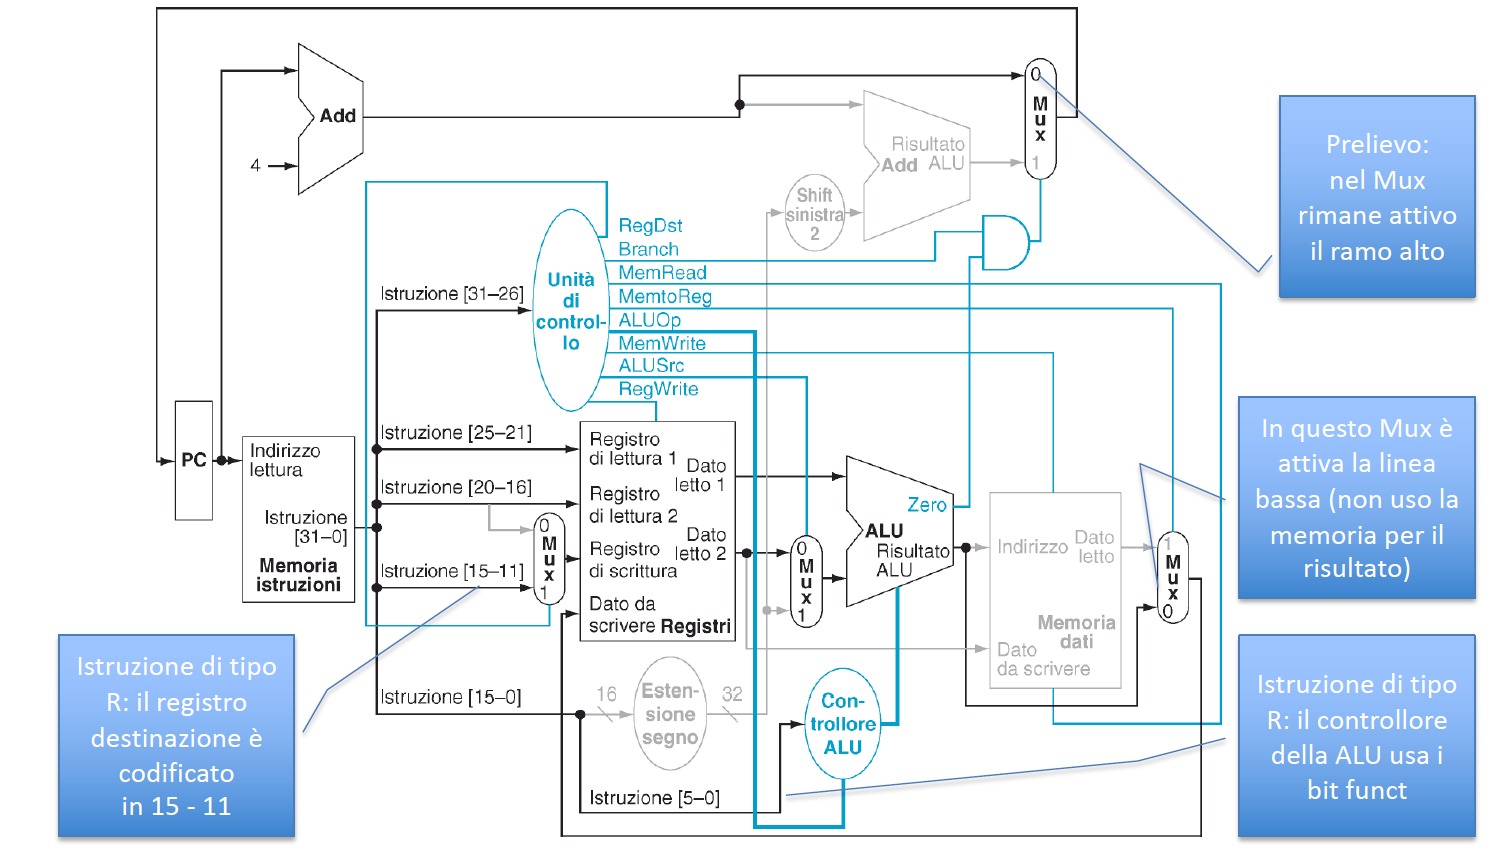
\includegraphics[width=0.95\textwidth,keepaspectratio]{es_add.png}
	\caption{Esecuzione di ADD sulla CPU}
\end{figure}

\subsubsection{Istruzione di LW}
Per eseguire un'istruzione di \opcode{lw} del tipo \mintinline{asm}{lw $t1, offset($t2)}, occorre:
\begin{enumerate}
	\item Prelevare l’istruzione dalla memoria e incrementare il \register{PC} di 4;
	\item Prelevare \register{\$t2} dal register file;
	\item Sommare \register{\$t2} ai campi offset dell’istruzione (i 16 bit meno significativi);
	\item L'indirizzo calcolato viene inviato alla memoria dati;
	\item Il dato all'indirizzo calcolato viene prelevato dalla memoria dati e memorizzato in \register{\$t1}.
\end{enumerate}
Si ricordi che l'insieme di tutte queste operazioni va eseguito in un unico ciclo di clock.

\begin{figure}[H]
	\centering
	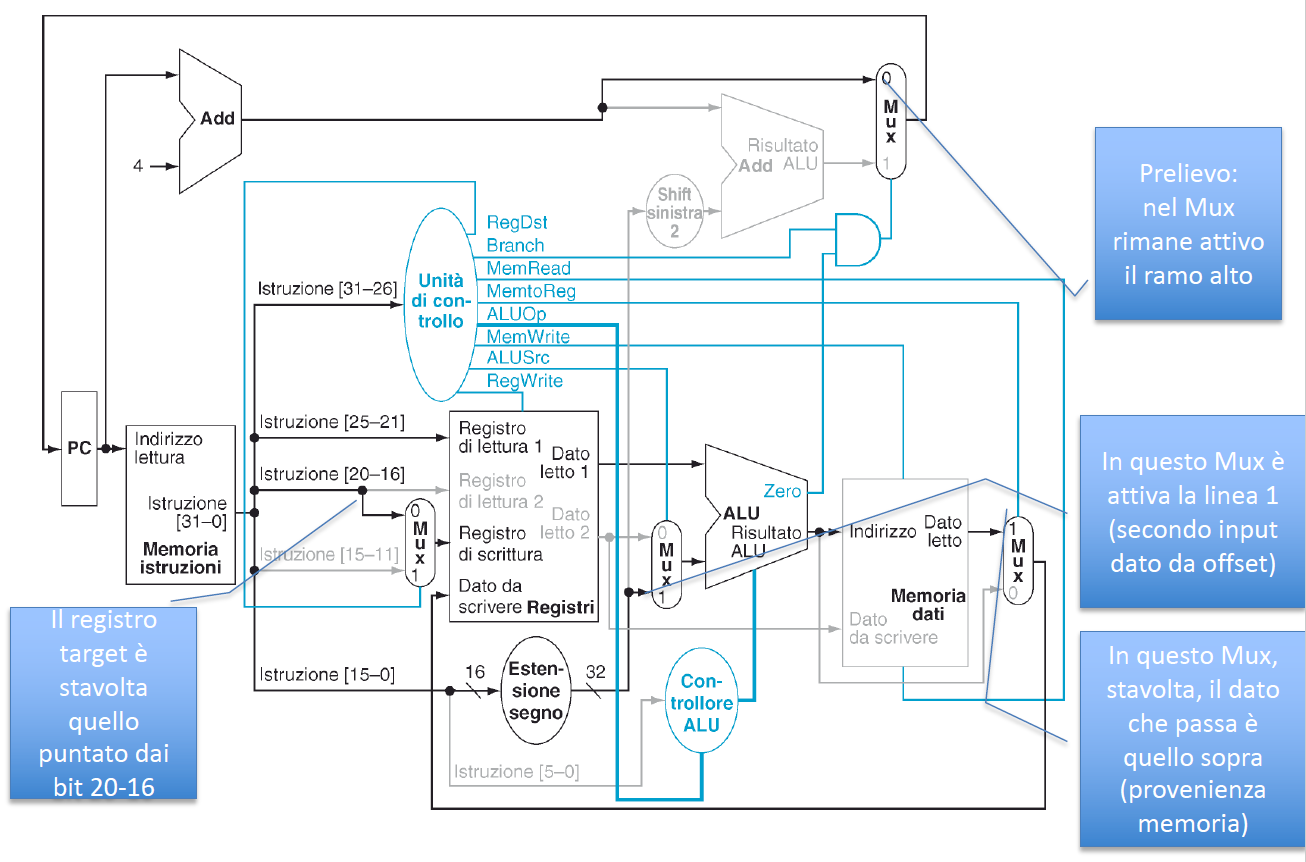
\includegraphics[width=0.95\textwidth,keepaspectratio]{es_lw.png}
	\caption{Esecuzione di LW sulla CPU}
\end{figure}

\subsubsection{Istruzione di BEQ}
Per eseguire un'istruzione di \opcode{beq} del tipo \mintinline{asm}{beq $t1, $t2, offset}, occorre:
\begin{enumerate}
	\item Prelevare l’istruzione dalla memoria e incrementare il \register{PC} di 4;
	\item Prelevare \register{\$t1} e \register{\$t2} dal register file;
	\item La ALU sottrae \register{\$t1} da \register{\$t2}. Il valore di \(\textrm{\emph{PC}}+4\) viene sommato all’offset (esteso a 32 bit) e shiftato di due volte (per indirizzare word e non in byte);
	\item Il codice di controllo \CUflag{zero} della ALU viene usato per decidere a cosa settare il \emph{PC}.
\end{enumerate}
Si ricordi che l'insieme di tutte queste operazioni va eseguito in un unico ciclo di clock.

\begin{figure}[H]
	\centering
	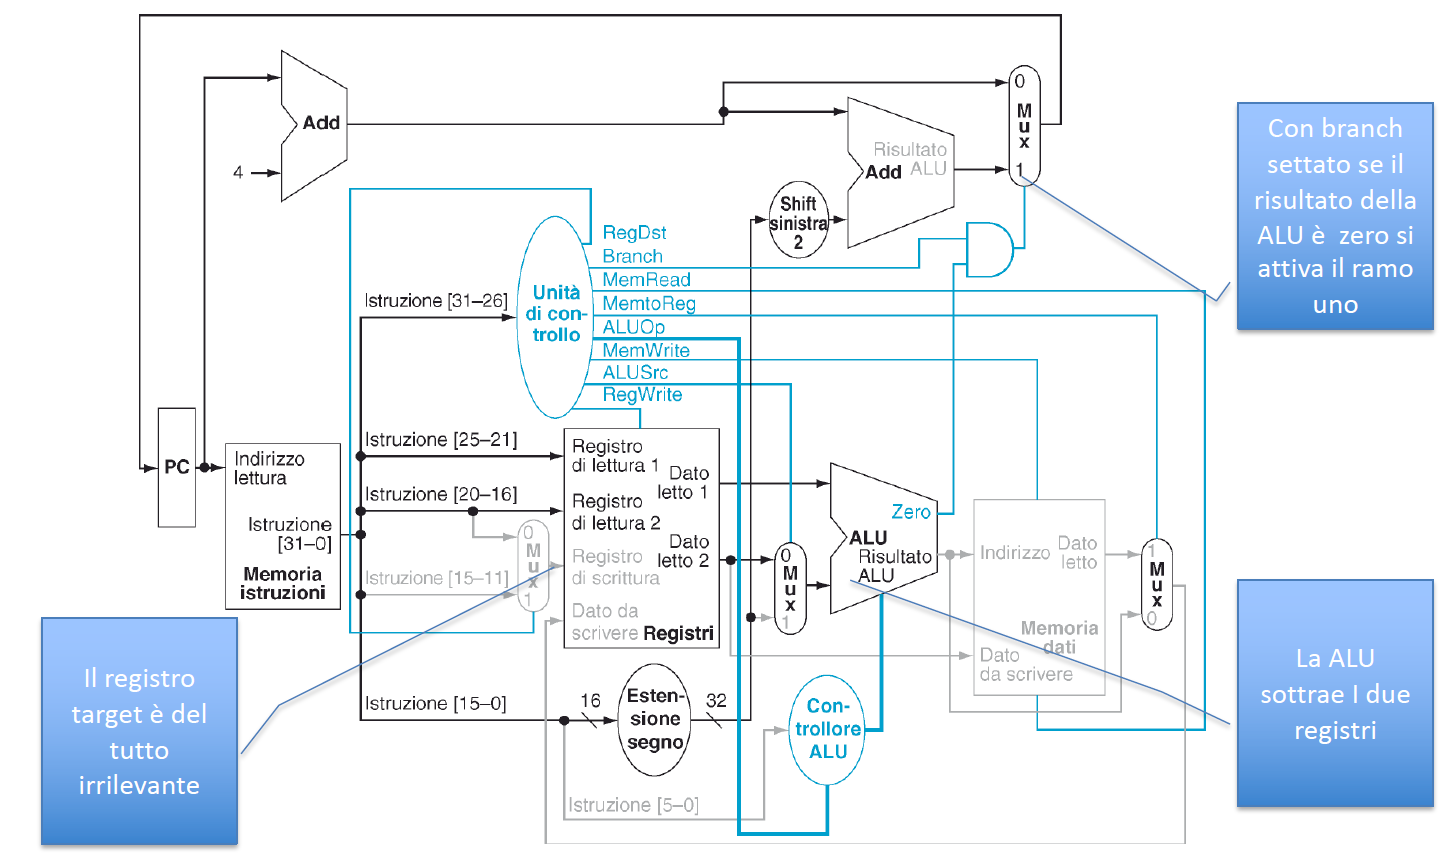
\includegraphics[width=0.95\textwidth,keepaspectratio]{es_beq.png}
	\caption{Esecuzione di BEQ sulla CPU}
\end{figure}

\subsubsection{Istruzione di J}
Per eseguire un'istruzione di \opcode{j} (salto incodizionato), occorre:
\begin{enumerate}
	\item Prelevare l’istruzione dalla memoria e incrementare il \register{PC} di 4;
	\item Sostituire al \register{PC} il nuovo valore così ottenuto:
	\begin{itemize}
		\item i quattro bit più significativi del \register{PC} rimangono invariati;
		\item i bit dal 27 al 2 (inclusi) del \register{PC} sono sostituiti con il campo indirizzo dell'istruzione \opcode{j};
		\item i due bit meno significativi sono messi a 0 (ragioniamo in word e non in byte).
	\end{itemize}
\end{enumerate}
Si ricordi che l'insieme di tutte queste operazioni va eseguito in un unico ciclo di clock.

\begin{figure}[H]
	\centering
	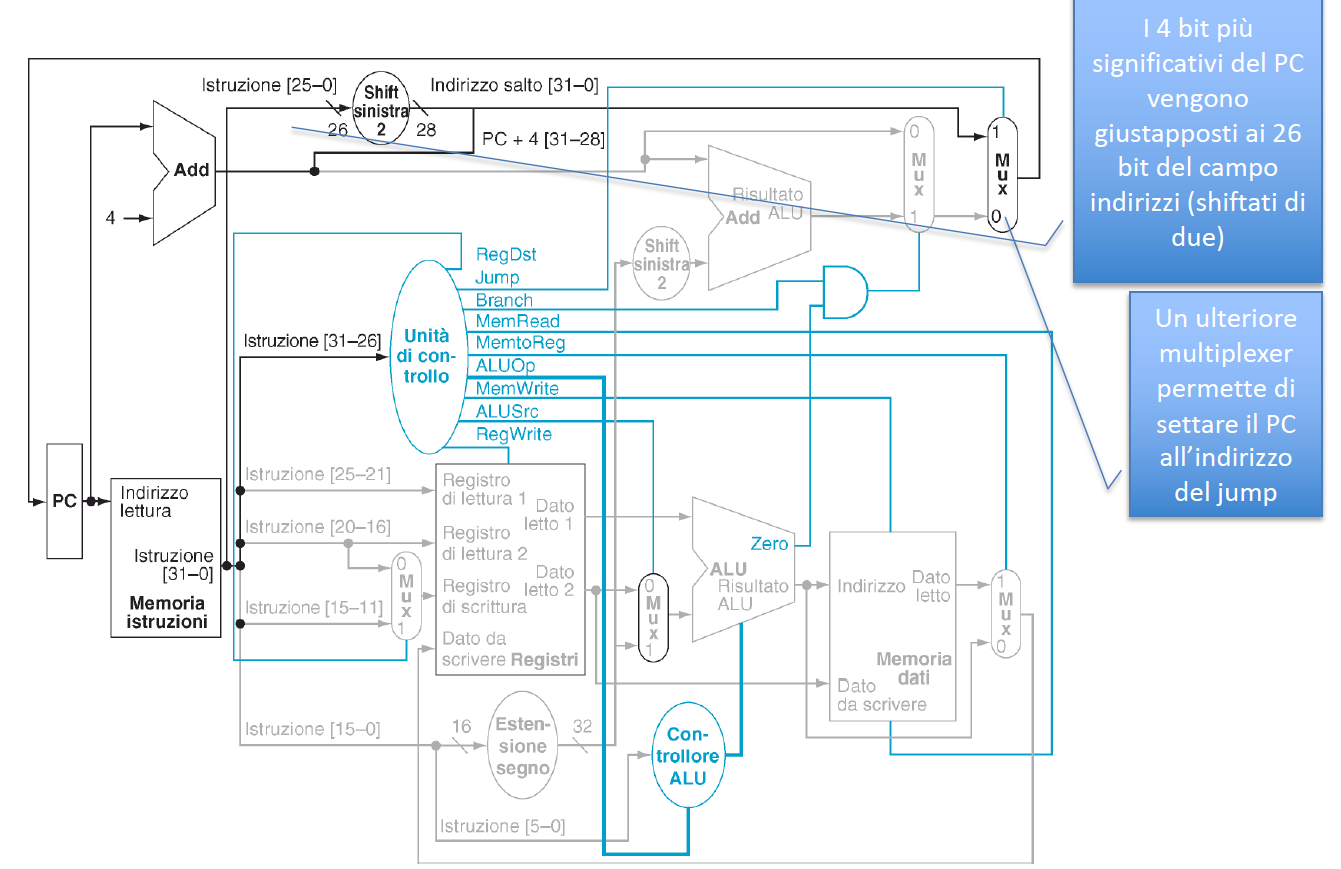
\includegraphics[width=0.95\textwidth,keepaspectratio]{es_j.png}
	\caption{Esecuzione di J sulla CPU}
\end{figure}

\subsection*{Conclusione}
Abbiamo appena visto come realizzare un semplice processore che esegue ciascuna delle istruzioni implementate in un singolo ciclo di clock. Solitamente però, si cerca di evitare un'implementazione di questo tipo, in quanto:
\begin{itemize}
	\item a dettare il clock sono le istruzioni più lente (solitamente l'operazione più costosa è quella per accedere alla memoria);
	\item più aumenta la complessità delle istruzioni da implementare, più la progettazione diventa complessa (esempio: istruzioni dedicate ai floating point);
	\item non è possibile fare ottimizzazioni aggressive sulle operazioni che avvengono più frequentemente.
\end{itemize}

\end{document}
